% =========================================================
%  Supplementary Material for:
%  Compact Offset-Free Interaction-Error MPC for pHRI
% =========================================================
\documentclass[journal]{IEEEtran}

\usepackage{amsmath,amssymb,amsfonts}
\usepackage{amsthm}
\usepackage{graphicx}
\usepackage{booktabs}
\usepackage{bm}
\usepackage{cite}
\usepackage[colorlinks=true,linkcolor=blue,citecolor=blue,urlcolor=blue]{hyperref}

\interdisplaylinepenalty=2500

\newtheorem{theorem}{Theorem}
\newtheorem{remark}{Remark}
\renewcommand{\thetheorem}{S\arabic{theorem}}
\renewcommand{\theremark}{S\arabic{remark}}

% Convenience macros (identical to phri_main.tex)
\newcommand{\Lam}{\Lambda(q)}
\newcommand{\Laminv}{\Lambda^{-1}(q)}
\newcommand{\Fmpc}{F_{\text{mpc}}}
\newcommand{\Fmpck}[1]{F_{\text{mpc},#1}}
\newcommand{\dhat}{\hat{d}}
\newcommand{\Jvb}{\bar{J}_v}
\newcommand{\Nbar}{\bar{N}}

\setlength{\textfloatsep}{6pt plus 2pt minus 2pt}
\setlength{\floatsep}{5pt plus 2pt minus 2pt}
\setlength{\intextsep}{5pt plus 2pt minus 2pt}
\setlength{\dbltextfloatsep}{7pt plus 2pt minus 2pt}
\setlength{\abovecaptionskip}{3pt}
\setlength{\belowcaptionskip}{0pt}
\setlength{\abovedisplayskip}{4pt plus 1pt minus 1pt}
\setlength{\belowdisplayskip}{4pt plus 1pt minus 1pt}
\setlength{\abovedisplayshortskip}{2pt plus 1pt}
\setlength{\belowdisplayshortskip}{2pt plus 1pt}

\begin{document}

\title{Supplementary Material: Compact Offset-Free Interaction-Error MPC
with Applied-Torque Constraints for Physical Human--Robot Interaction}

\author{Yongyan~Cao$^{1}$ and Jinshan~Tang$^{2}$%
\thanks{$^{1}$Y. Cao is with Voryx Robotic LLC, San Jose, CA 95136, USA
(e-mail: yongyancao@gmail.com).}%
\thanks{$^{2}$J. Tang is with the Department of Health Administration and
Policy, George Mason University, Fairfax, VA, USA
(e-mail: jtang25@gmu.edu).}}

\maketitle

\begin{abstract}
This document accompanies the main paper and contains: the full
controllability/detectability argument and LMI-based stabilizability
proof for the LPV backbone, the parameter table, and additional
experiments that supplement, but are not required to follow, the main
paper's core argument --- the waypoint-hold benchmark (redundant with
Benchmark~I's conclusions), the time-varying-force horizon-prediction
study, the human-force magnitude/shape sweep, and the impedance-backbone
correction-authority ablation. Table numbers here are prefixed ``S'' and
are independent of the main paper's numbering.
\end{abstract}

% ----------------------------------------------------------
\section{Controllability and Detectability of the LPV Backbone}\label{sec:controllability}

\begin{remark}[Controllability and Detectability]\label{rem:feasibility}
The LPV system (8) of the main paper is uniformly controllable across
all configurations $\rho_k$ in the singularity-free workspace. Since
$\Lambda(q)$ in eq.~(2) is symmetric positive-definite for all $q$ away
from kinematic singularities, $\Laminv$ is full rank, so $B_d(\rho_k)$
has full column rank 3 (via its velocity block). With $A_d$ mixing
velocity into position, the position rows of $B_d$ and $A_dB_d$ differ
by $-\Laminv\Delta t^2$ (full rank), so the controllability matrix
$\mathcal C=[B_d\mid A_dB_d]$ has rank 6 for all $\rho_k$. If
$Q\succeq0$, $R\succ0$, and $(Q^{1/2},A_d)$ is detectable, the discrete
algebraic Riccati equation (DARE) admits a stabilizing solution at every
fixed configuration, and the infinite-horizon LQR gain
\begin{equation*}
K_\infty=(R+B_d^\top P_\infty B_d)^{-1}B_d^\top P_\infty A_d
\end{equation*}
is well-defined everywhere. For the augmented estimator, observability
of $[e;\dot e]$ together with full column rank of $B_d$ makes the
constant disturbance state detectable: if a mode is unobservable from
$C=[I_6\ 0]$, its $x_e$ component is zero; the augmented dynamics then
require $B_dd=0$, hence $d=0$.
\end{remark}

This is the basis for Corollary~1's DARE-solvability claim and for the
LPV-backbone stabilizability result of Sec.~\ref{sec:stab}.

% ----------------------------------------------------------
\section{Common-Quadratic Stabilizability of the Scheduled Error Predictor}\label{sec:stab}

\begin{theorem}[Quadratic Stabilizability of the Scheduled Error
Predictor]\label{thm:workspace}
Consider the LPV error predictor
$x_{e,k+1}=A_dx_{e,k}+B_d(\rho_k)\Fmpck{k}$ with constant $A_d$ and
$B_d(\rho)$ as in eq.~(8) of the main paper, and suppose the
operational-space inverse-inertia stays in a compact polytope over the
operating region of interest,
$\Laminv\in\mathcal P=\operatorname{conv}\{L_1,\dots,L_V\}$ (e.g.\ the
entry-wise box with $0\prec\lambda_{\min}I\preceq\Laminv\preceq\lambda_{\max}I$)
--- a certified bound on $\Laminv$, either established analytically over
the entire singularity-free workspace or, as instantiated in
Remark~\ref{rem:instantiation} below, sampled over a specific operating
region --- with vertex input matrices
$B_v=[-\tfrac{\Delta t^2}2L_v;\,-L_v\Delta t]$ (affine in $\Laminv$, so
the polytope structure is preserved). If there exist $Q=Q^\top\succ0$ and
$Y\in\mathbb R^{3\times6}$ and a prescribed $0<\varrho<1$ such that, for
every vertex $v=1,\dots,V$,
\begin{equation}
\begin{bmatrix}\varrho^2Q & (A_dQ+B_vY)^\top\\A_dQ+B_vY & Q\end{bmatrix}\succ0,
\label{eq:lmi}
\end{equation}
then the \emph{fixed} state-feedback law $\Fmpc=Kx_e$ with $K=YQ^{-1}$
makes $V(x)=x^\top Px$, $P=Q^{-1}$, a \emph{common} quadratic Lyapunov
function: $V(x_{e,k+1})<\varrho^2V(x_{e,k})$ for
\emph{every} admissible configuration trajectory
$\{\rho_k\}\subset\mathcal P$, so this one fixed linear feedback law is
exponentially stabilizing uniformly over $\mathcal P$ --- not only at a
frozen configuration. This is a statement about the LPV \emph{backbone}
under a single certified feedback gain, not directly about the
finite-horizon receding-horizon MPC actually deployed (see the scope
remark below).
\end{theorem}

\begin{proof}
$B_d(\rho)$ is affine in $\Laminv[\rho]$, so for any $\rho$ with
$\Lambda^{-1}(\rho)=\sum_v\alpha_vL_v$ ($\alpha_v\ge0$,
$\sum_v\alpha_v=1$) we have
$A_dQ+B_d(\rho)Y=\sum_v\alpha_v(A_dQ+B_vY)$. The block matrix in
\eqref{eq:lmi} is affine in this quantity, and the positive-definite
cone is convex, so \eqref{eq:lmi} holds for all $\rho\in\mathcal P$, not
only at the vertices. Taking the Schur complement of the lower-right
block gives
$(A_dQ+B_d(\rho)Y)^\top Q^{-1}(A_dQ+B_d(\rho)Y)\prec\varrho^2Q$.
Writing $A_\text{cl}(\rho)=A_d+B_d(\rho)K$ with $K=YQ^{-1}$ and
pre/post-multiplying by $Q^{-1}=P$ yields
$A_\text{cl}(\rho)^\top PA_\text{cl}(\rho)-\varrho^2P\prec0$, for
all $\rho\in\mathcal P$. Hence $V(x)=x^\top Px$ decreases along every
trajectory regardless of how $\rho_k$ varies, which is exponential
stability of this fixed-gain LPV closed loop. Composing with the
detectable integrating-disturbance estimator of Theorem~2 of the main
paper, the tracking error is offset-free at each constant-contact
equilibrium the trajectory visits, \emph{for this fixed-gain closed
loop}.
\end{proof}

This is the polytope-level counterpart of the per-configuration DARE
solvability of Remark~\ref{rem:feasibility} and the continuous scheduled
law of Corollary~1 of the main paper: it certifies that the
interaction-error \emph{representation} --- enabled by the constant
$A_d$, which confines all configuration variation to the affine
$B_d(\rho)$ and makes \eqref{eq:lmi} a finite vertex program --- is
quadratically stabilizable by a single Lyapunov function over
$\mathcal P$, under one fixed certified gain.

\textbf{Scope.} Theorem~\ref{thm:workspace} establishes exponential
stability of the \emph{nominal predictive backbone under one fixed,
LMI-certified linear feedback gain} --- the disturbance-free LPV closed
loop $(A_d,B_d(\rho))$, with the input constraint inactive --- not
workspace-wide stability of the complete deployed controller. In
particular it does \textbf{not} by itself analyze: the disturbance
estimator (offset-free tracking under the Kalman estimator is Theorem~2
of the main paper's separate result, composed with
Theorem~\ref{thm:workspace} only informally, in the last line of the
proof above); the finite-horizon receding-horizon re-solve, whose
realized policy at each step is the QP's actual minimizer, not the
certified fixed $K$ (the unconstrained QP realizes \emph{a} member of
this same class of linear state feedback, Theorem~1/Corollary~1 of the
main paper, but not necessarily the specific certified $K$); or the
safety and passivity filters (Theorem~3, Proposition~2 of the main
paper). The complete controller's closed-loop guarantees are therefore
this \emph{collection} of separately-scoped results about different
feedback laws, not one monolithic proof that the deployed MPC is
workspace-stable.

\begin{remark}[Rate-independence and the frozen horizon]
The certificate uses a \emph{single, parameter-independent} Lyapunov
matrix $P=Q^{-1}$ shared by all vertices. A common-$P$ quadratic-stability
certificate is robust to \emph{arbitrary} time variation of
$\rho_k\in\mathcal P$ --- including arbitrarily fast changes --- with no
assumption on the parameter-variation rate $\|\rho_{k+1}-\rho_k\|$: the
Lyapunov decrease holds at every vertex and hence, by convexity of
\eqref{eq:lmi} in $\Laminv$, for any $\rho_k\in\mathcal P$ regardless of
how it moves, \emph{provided the certified fixed $K$ is what is actually
applied}. This gives a \emph{structural reason}, not a proof, for why the
frozen-$\Gamma$ approximation used online (built from the current
$B_d(q_k)$ and held over the $N$-step horizon) is unlikely to be
destabilizing: the gap between $B_d(q_k)$ and the true future
$B_d(q_{k+i})$ is a bounded variation \emph{inside} $\mathcal P$, and a
fixed-$K$ closed loop over $\mathcal P$ would not be destabilized by that
variation regardless of its rate. This motivates, but does not
establish, that the deployed receding-horizon policy --- which re-solves
a QP rather than applying the certified $K$ --- inherits the same
robustness; the frozen horizon shapes only the \emph{predicted}
trajectory, while the receding-horizon re-solve keeps the
\emph{applied} first move matched to the current $\rho_k$, but no result
in this paper proves the resulting closed loop shares
Theorem~\ref{thm:workspace}'s rate-independence.
\end{remark}

\begin{remark}[Numerical instantiation of $\mathcal P$]\label{rem:instantiation}
For the FR3, sampling $\Laminv$ along the main paper's \S V circular
benchmark (4700 samples) gives
$\operatorname{eig}\Laminv\in[0.059,0.354]\ \text{kg}^{-1}$ (task
inertia 2.8--16.9\,kg). The resulting entry-wise box has 64 corners in
general, but not every corner of an independent per-entry box need be
positive-definite; we discard any that are not (none were, here --- all
64 corners were confirmed SPD, minimum eigenvalue $\approx0.023\
\text{kg}^{-1}$ across vertices, comfortably above the regularization
floor). Direct entry-wise auditing reports zero containment violation for all
4700 samples. This instantiates $\mathcal P$ over the \emph{sampled operating
region traversed by the benchmark trajectory}, not a verified bound over
the entire singularity-free workspace; extending the certified range to
other trajectories or the full workspace would need re-sampling or an
analytic eigenvalue bound, neither done here. Over this $\mathcal P$
($\Delta t=10$\,ms), the minimum-condition-number common-$P$ certificate
at guaranteed rate $\rho\le0.996$ is feasible, returning a
well-conditioned common $P$ ($\operatorname{cond}P\approx2.2$) with
spectral radius $\le0.996$ and strictly negative Lyapunov increment
($\max\operatorname{eig}(A_\text{cl}^\top PA_\text{cl}-P)\approx-5\times10^{-3}$)
at every vertex. For the exact-ZOH model, CLARABEL reports
\texttt{optimal}; the target-rate residual
$\max\operatorname{eig}(A_\text{cl}^\top PA_\text{cl}-0.996^2P)$ is
$-9.0\times10^{-7}$ and the minimum eigenvalue of the LMI block is
$9.9\times10^{-7}$. These checks apply \emph{for the certified fixed
$K=YQ^{-1}$} --- the
realized MPC, with its far larger tracking weights and different
(receding-horizon) policy, is not shown to converge at this rate, only
observed empirically to converge faster. This establishes the
qualitative backbone-stabilizability claim rigorously over the sampled
region rather than empirically, and is reproducible from the released
script (\texttt{lmi\_workspace\_stability\_probe.py}).
\end{remark}

% ----------------------------------------------------------
\section{Parameters}\label{sec:params}

Every numeric constant used across the experiments of the main paper
(\S VI) and this supplement is consolidated below, cross-checked against
the released files \path{simulation/impedance_mpc.py},
\path{simulation/phri.py}, and
\path{cloud_verify/lib/fr3_hardware_interface.py} rather than
restated from memory. Unless a table or figure caption states otherwise,
these are the values used throughout.

\begin{table}[!t]
\caption{Controller and Estimator Parameters}
\label{tab:params}
\renewcommand{\arraystretch}{1.0}
\footnotesize
\setlength{\tabcolsep}{3pt}
\begin{tabular}{p{2.3cm}p{1.2cm}p{2.5cm}}
\toprule
\textbf{Parameter} & \textbf{Symbol} & \textbf{Value}\\
\midrule
Prediction horizon & $N$ & 10\\
MPC sample time (100\,Hz) & $\Delta t$ & 10\,ms\\
MPC sample time (500\,Hz) & $\Delta t$ & 2\,ms\\
Inner-loop rate & --- & 1\,kHz\\
Position stage weight & $Q_\text{pos}$ & $2\times10^4 I_3$\\
Velocity stage weight & $Q_\text{vel}$ & $50\,I_3$\\
Terminal cost scale & $\gamma$ & 5\\
Effort weight & $R$ & $10^{-6}I_3$\\
Corrective-force bound & $F_\text{max}$ & 150\,N\\
FR3 torque limits & $\tau_\text{max}$ & $87\!\times\!4;\ 12\!\times\!3$\,Nm\\
$\Lambda^{-1}$ regularization & $\sigma$ & $10^{-6}$\\
Kalman process noise & $Q_d$ & 10.0\\
Kalman obs.\ noise (pos.) & --- & $10^{-3}$\\
Kalman obs.\ noise (vel.) & --- & $10^{-2}$\\
Orientation stiffness & $K_\text{rot}$ & 20\,Nm/rad\\
Orientation damping & $D_\text{rot}$ & 6\,Nm$\cdot$s/rad\\
Null-space centering stiffness & $k_\text{null}$ & 10\,Nm/rad\\
Null-space damping & $d_\text{null}$ & 2\,Nm$\cdot$s/rad\\
Null-space barrier gain & $k_b$ & 50\,Nm\\
Barrier activation threshold & $\eta$ & 0.10\\
Workspace-projection gain & $k_\text{ws}$ & $5\times10^{-4}$ m/(Nm/rad)$^\dagger$\\
Workspace-projection cap & $p_\text{max}$ & 0.06\,m\\
Workspace-projection reg. & $\epsilon_r$ & $10^{-8}$\\
Backbone stiffness (C8) & $K_\text{bb}$ & 300\,N/m\\
Backbone damping ratio (C8) & $\zeta_\text{bb}$ & 1.0 (nominal)\\
CBF safety margin & $\epsilon$ & 0.05\,rad\\
CBF contraction rate & $\alpha$ & 0.5\\
CBF slack penalty weight & $w_s$ & $10^{8}$\\
Tank initial energy & $E_0$ & 20.0\,J\\
Tank lower bound & $E_\text{min}$ & 0.05\,J\\
Tank upper bound & $E_\text{max}$ & 50.0\,J\\
Human-recharge fraction & $\gamma$ (tank) & 0.0\\
OSQP tolerances & abs., rel. & $10^{-6}$\\
OSQP iteration cap & --- & 4000\\
Circular benchmark $R,T$ & --- & 0.12\,m, 8\,s\\
Human step force & $F_h$ & 15\,N, $t\in[3,6]$\,s\\
Reference ramp time & $T_\text{ramp}$ & 1.5\,s\\
FR3 neutral pose & $q_0$ &
$\begin{array}{c}[0,-0.785,0,\\-2.356,0,1.571,\\0.785]\end{array}$ rad\\
\bottomrule
\end{tabular}
\end{table}

Two parameter sets are estimator/CBF-internal and are not separately
swept: the Kalman noise covariances and the CBF/tank constants (the
latter are exercised in the \texttt{cloud\_verify} hardware-path suite
rather than the direct benchmark scripts used for the main paper's
tables).

$^\dagger$Benchmarks I and II in the main paper are run with
$k_\text{ws}=0$: the driver scripts
for those two circular/waypoint benchmarks disable workspace projection
so its effect does not confound the controller-to-controller
comparison. The $5\times10^{-4}$ default above is what the boundary
test in the main paper actually uses, which is where the
mechanism is exercised and discussed.

% ----------------------------------------------------------
\section{Focused Fair-Comparison Protocol}\label{sec:fair}

The focused comparison in the main paper separates calibration from testing.
Calibration uses one 8\,s cycle; after selecting parameters, every reported
metric is recomputed in a newly reset environment over three cycles (24\,s).
No test-cycle metric enters parameter selection. The response-matched
impedance first uses $K_0=\|F_h\|/\|e_{\rm ss,C4}\|=5441$\,N/m, then evaluates
the Cartesian product
\[
K/K_0\in\{0.8,1.0,1.2\},\qquad
\zeta\in\{0.7,1.0,1.3\}.
\]
The score is contact-onset trajectory RMSE relative to C4 plus absolute
steady-state-error mismatch; $K=5441$\,N/m, $\zeta=1.3$ is selected. The
anti-windup PI grid is
\[
K_i\in\{120,300,700\},\qquad
I_{\max}\in\{0.02,0.06,0.12\}\ \text{m\,s},
\]
with score $e_{\rm ss}+0.25e_{\rm RMS,contact}+0.01r_{\rm sat}$; it selects
$K_i=120$ and $I_{\max}=0.02$\,m\,s. The complete 18-run calibration ledger,
selected scores, test metrics, QP counts, and saturation diagnostics are stored
in \path{simulation/fair_offset_free_comparison.json} and regenerated by
the identically named Python script.

The measured-force comparator uses the response-matched impedance and receives
the exact applied simulation wrench through a first-order filter
($T_f=50$\,ms), commanding $-J_v^\top\hat F_h$ in the same Cartesian force
channel through which $F_h$ enters. It reaches 1.39\,mm total steady-state
error (0.50\,mm on the force axis), so it confirms rather than denies that
current-step force cancellation rejects a constant load. Unlike C5, however,
it assumes a direct force measurement. ``Saturation'' in this experiment means
a raw magnitude-limit excess above $10^{-3}$\,Nm. Both MPC variants have zero
failed solves in 2400 updates and maximum raw excess below
$2\times10^{-5}$\,Nm; neither uses the CBF, tank, or torque-rate filter in this
focused script.

% ----------------------------------------------------------
\section{Four-Plane Circle Tracking}\label{sec:planes}

C5 (MPC + Kalman, 100\,Hz QP, 1\,kHz inner) is evaluated on four 3-D
circle planes, complementing the XZ-plane result of Benchmark~I.
Table~\ref{tab:planes} reports RMSE after the 1.5\,s ramp.

\begin{table}[!t]
\caption{Free-Space Circle Tracking, $R=12$\,cm, $T=8$\,s}
\label{tab:planes}
\renewcommand{\arraystretch}{1.0}
\centering
\setlength{\tabcolsep}{4pt}
\footnotesize
\begin{tabular}{@{}lccc@{}}
\toprule
\textbf{Plane} & \textbf{IMP RMSE [mm]} & \textbf{MPC RMSE [mm]} & \textbf{Improvement}\\
\midrule
XZ sagittal  & 23.54 & 0.24 & $\times$97\\
XY horizontal & 25.06 & 0.33 & $\times$77\\
YZ frontal   & 16.25 & 0.20 & $\times$79\\
XZ$\to$XY tilted & 25.07 & 0.31 & $\times$80\\
\bottomrule
\end{tabular}
\end{table}

\textbf{Analysis.} The MPC maintains sub-0.35\,mm RMSE across all
planes, demonstrating that the $\Lam$-adaptive compliance in the QP
(eq.~9 of the main paper) handles the off-diagonal operational-space
inertia coupling without gain scheduling --- the controller was tuned
and validated on the XZ plane alone (Benchmark~I), and the other three
planes are a held-out generalization check, not a separately re-tuned
result.

% ----------------------------------------------------------
\section{Benchmark II --- Reach-and-Hold under Human Push}\label{sec:bm2}

\textbf{Scenario.} The robot navigates a triangle of three waypoints (A,
B, C) in one lap. At each waypoint, 0.8\,s after arrival, a directionally
varied 15\,N push fires for 2\,s. The robot must recover and dwell
within 35\,mm of the target for 1\,s before advancing (3 push events, one
per waypoint).

\begin{figure}[!t]
\centering
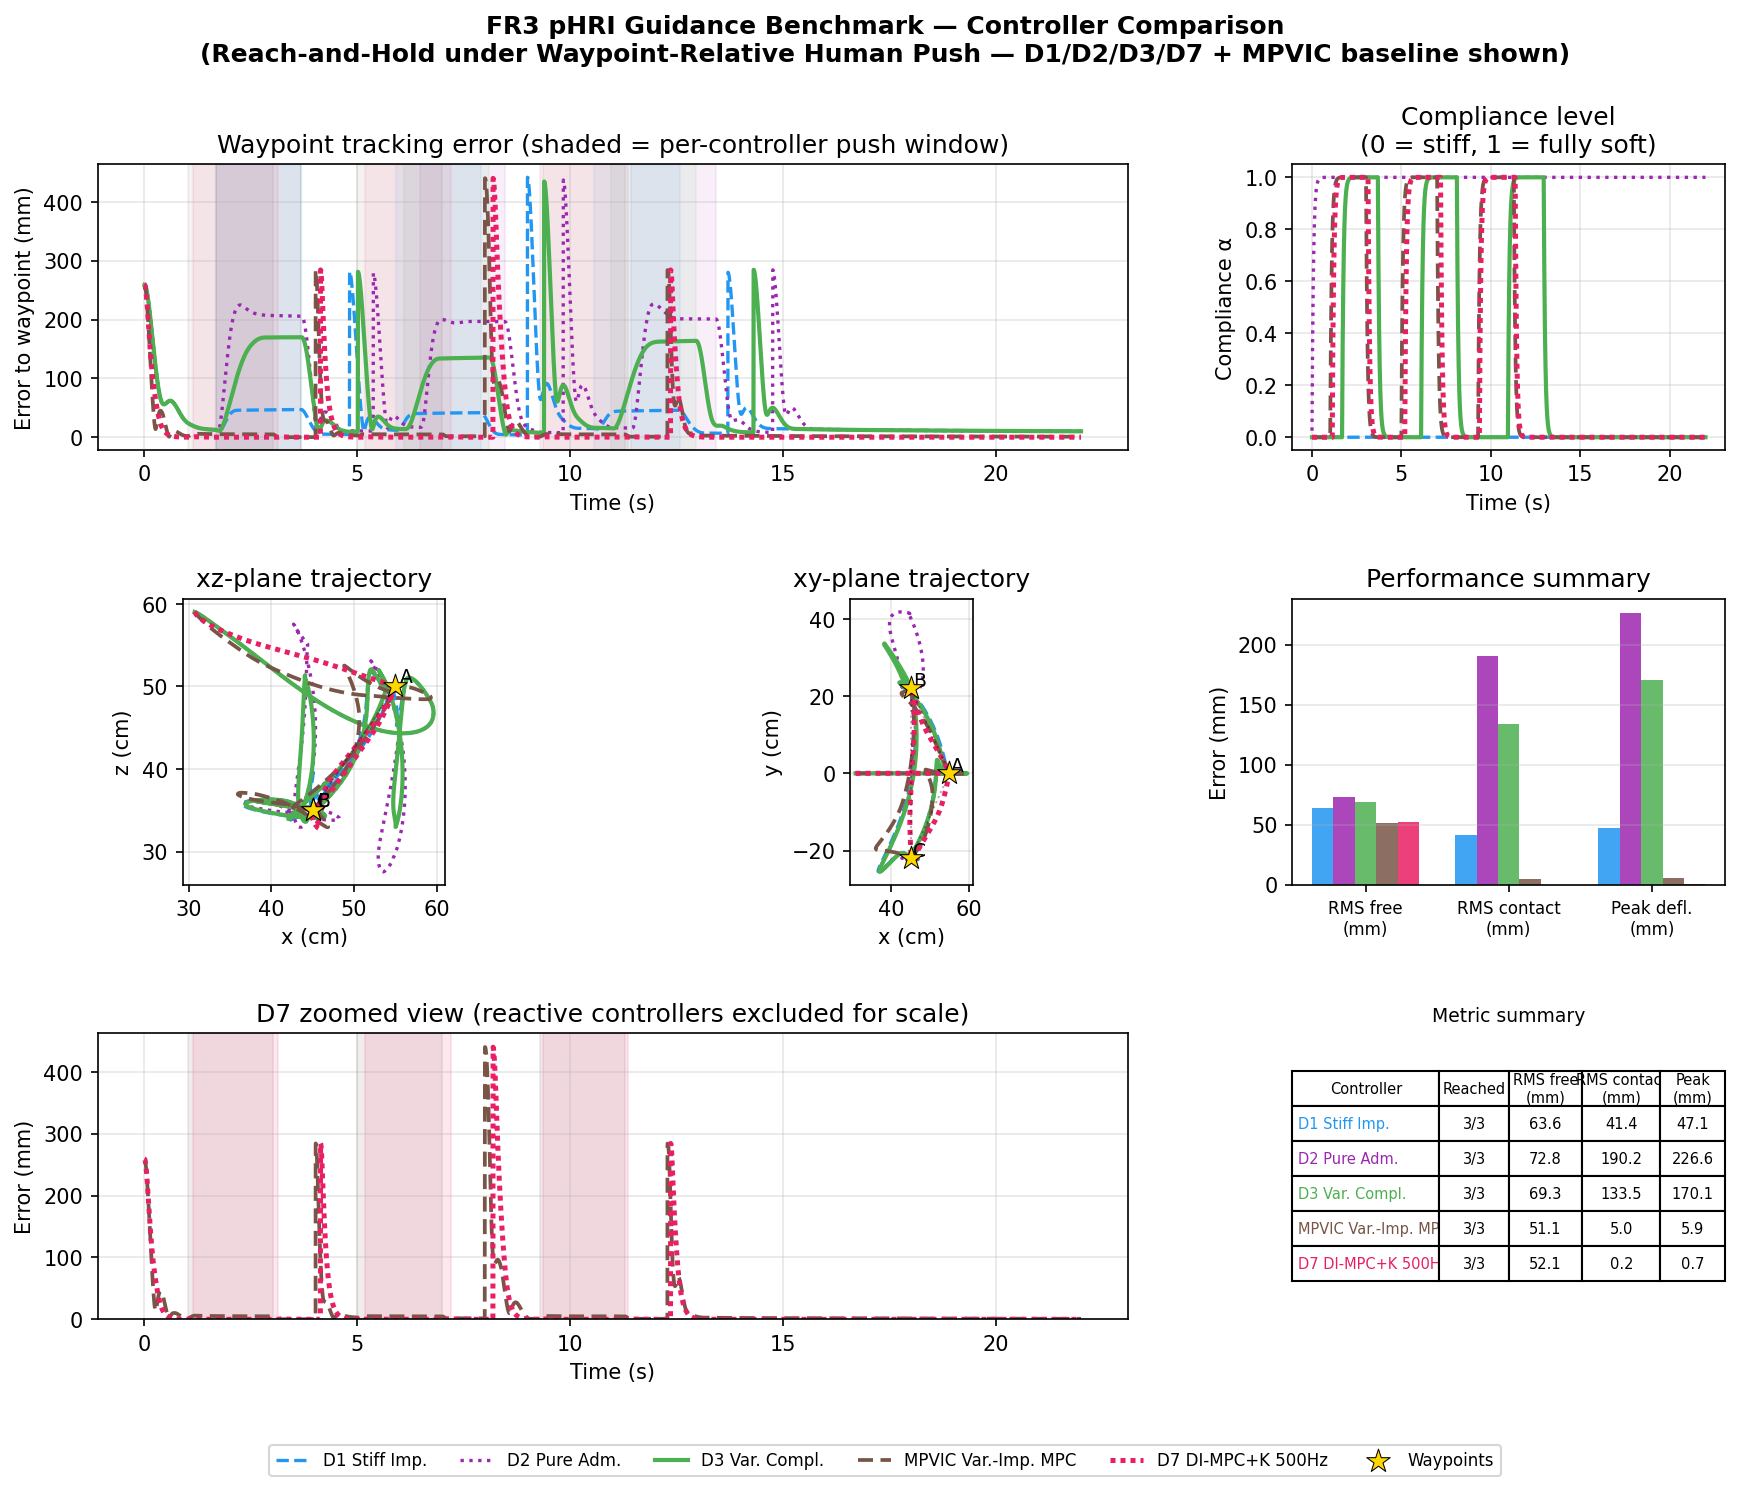
\includegraphics[width=0.85\columnwidth]{figures/guidance_controller_comparison.png}
\caption{Benchmark II --- reach-and-hold under directionally varied
push. For visibility the plot shows D1/D2/D3/D7 (corresponding to
G1/G2/G3/G7) plus the predictive variable-impedance MPVIC baseline;
Table~\ref{tab:bm2} reports the full ablation. The final D7 controller
reaches every waypoint with sub-millimeter contact-window deflection.}
\label{fig:bm2}
\end{figure}

\begin{table}[!t]
\caption{Benchmark II: Waypoint-Hold Under Directionally Varied Push}
\label{tab:bm2}
\renewcommand{\arraystretch}{1.0}
\footnotesize
\setlength{\tabcolsep}{3pt}
\begin{tabular}{lcccc}
\toprule
\textbf{Controller} & \textbf{Waypts} & \textbf{RMS free} & \textbf{RMS cont.} & \textbf{Peak}\\
\midrule
G1 -- Stiff Impedance    & 3/3 & 63.6 & 41.4 & 47.1\\
G2 -- Pure Admittance    & 3/3 & 72.8 & 190.2 & 226.6\\
G3 -- Variable Compl.    & 3/3 & 69.3 & 133.5 & 170.1\\
MPVIC -- Var.-Imp. MPC   & 3/3 & 51.2 & 5.0 & 6.0\\
G4 -- MPC 100\,Hz        & 3/3 & 47.9 & 2.2 & 2.6\\
G5 -- MPC+K 100\,Hz      & 3/3 & \textbf{47.9} & 0.6 & 2.4\\
G6 -- MPC 500\,Hz        & 3/3 & 51.9 & 0.8 & 1.0\\
G7 -- MPC+K 500\,Hz      & 3/3 & 51.4 & \textbf{0.2} & \textbf{0.8}\\
\bottomrule
\end{tabular}
\end{table}

\textbf{Analysis.} The static-waypoint hold confirms the same separation
seen in Benchmark~I, and is included here for completeness rather than
as an independent finding. All four MPC variants (G4--G7) reach every
waypoint with order-of-magnitude lower contact-window deflection than
the reactive baselines: against the stiff-impedance baseline (G1), the
MPC cuts contact-window RMS from 41.4\,mm to 2.2\,mm (G4) and peak
deflection from 47.1\,mm to 2.6\,mm. Adding the Kalman augmentation
improves the contact and free-motion metrics --- G5 lowers contact-window
RMS from 2.2\,mm to 0.6\,mm and slightly reduces peak (2.6$\to$2.4\,mm)
--- so unlike a higher impedance gain it carries no peak penalty. Raising
the QP rate to 500\,Hz then sharpens the first-contact transient
further: G7 attains 0.2\,mm contact-window RMS and a 0.8\,mm peak. The
pure-admittance and variable-compliance baselines (G2, G3) yield by
design, producing the large 190--134\,mm contact-window deflections
expected of intentional compliance. The predictive variable-impedance
baseline (MPVIC) behaves oppositely to the reactive variable-compliance
G3: instead of softening, it stiffens predictively to reject the push,
cutting contact-window RMS to 5.0\,mm, yet it stays a further order of
magnitude above the offset-free G5 (0.6\,mm) --- the same non-offset-free
residual seen in Benchmark~I. As in Benchmark~I, MPVIC here is our own
discrete-stiffness scheduler, not a reproduced published algorithm; see
the main paper's Benchmark~I discussion for the corresponding caveat.

% ----------------------------------------------------------
\section{Time-Varying Interaction and Horizon-Prediction Validity}\label{sec:tv}

The benchmarks in the main paper apply constant or step forces. Because
the framework targets \emph{interaction} dynamics broadly, we
additionally exercise a \emph{time-varying} human force and measure a
proxy for the $N$-step disturbance-prediction RMS $\varepsilon_N$ of
Section~III-D of the main paper --- the quantity that bounds how well the
flat random-walk prediction holds over the horizon. To isolate the
effect of the force alone from configuration-driven terms, the robot
holds a \emph{static} target while a sinusoidal push
$F_z=-A\sin(2\pi ft)$ of fixed amplitude $A=12$\,N and increasing
frequency $f$ is applied, sweeping the disturbance rate
$L_d=A\,2\pi f/\sqrt2$. The controller is DI-MPC + Kalman (C5, 100\,Hz
QP).

\textbf{What $\varepsilon_N$ actually measures here.} Because the true
disturbance $d_k$ is not directly logged in this experiment, we use the
filtered estimate $\dhat_{k|k}$ as its proxy and the flat prediction
$\dhat_{k|k-N}=\dhat_{k-N|k-N}$, so
$\varepsilon_N=\mathrm{RMS}_k\|\dhat_{k|k}-\dhat_{k-N|k-N}\|$ measures
the $N$-step \emph{self-consistency of the estimate}, not the main
paper's eq.~(13) prediction error against the true $d_k$ directly ---
the two agree only to the extent $\dhat$ has converged to $d$. This is
visible in the $L_d=0$ (constant-force) row: the theoretical
extrapolation term $L_dN\Delta t$ is exactly zero there, yet the
measured $\varepsilon_N-\varepsilon_1=0.34$\,N is not --- that residual
is the estimator's own process-noise jitter accumulated over $N$ steps,
a real but different quantity from the extrapolation term. Table~\ref{tab:tv}
should therefore be read as evidence \emph{consistent with} the
linear-in-rate scaling eq.~(13) predicts, not a direct validation
against ground truth; a true ground-truth check --- computing $d_{a,k}$
from the logged simulation dynamics ($\ddot e_k+\Laminv\Fmpck{k}$, both
already available since the injected force is known) rather than the
filtered estimate --- is a well-defined follow-up we have not run.

\begin{table}[!t]
\caption{Time-Varying Force: Horizon Self-Consistency Error (Estimator
Proxy) and Tracking}
\label{tab:tv}
\renewcommand{\arraystretch}{1.0}
\footnotesize
\setlength{\tabcolsep}{3pt}
\begin{tabular}{cccccc}
\toprule
$L_d$ [N/s] & $\varepsilon_1$ & $\varepsilon_N$ & $\varepsilon_N{-}\varepsilon_1$ & Bound & RMS [mm]\\
\midrule
0.0  & 0.04 & 0.38 & 0.34 & 0.00 & 0.08\\
5.3  & 0.05 & 0.52 & 0.46 & 0.53 & 0.12\\
10.7 & 0.12 & 1.20 & 1.08 & 1.07 & 0.27\\
21.3 & 0.25 & 2.47 & 2.22 & 2.13 & 0.54\\
42.7 & 0.49 & 4.87 & 4.38 & 4.27 & 1.03\\
\bottomrule
\end{tabular}
\end{table}

\textbf{Analysis.} The measured horizon-extrapolation gap
$\varepsilon_N-\varepsilon_1$ (self-consistency proxy) tracks the bound
term $L_dN\Delta t$ to within $\approx10\%$ across a decade of
disturbance rate (0.46 vs.\ 0.53; 1.08 vs.\ 1.07; 2.22 vs.\ 2.13; 4.38
vs.\ 4.27\,N), consistent with the flat-prediction error being
\emph{linear in the force rate} as eq.~(13) predicts, with a
constant-force floor $\approx0.38$\,N (the $f=0$ row) set by the
estimate's process-noise jitter accumulated over the $N$ steps --- not
itself a prediction-error measurement (see above). Tracking degrades
gracefully: the controller holds sub-millimeter error up to
$L_d\approx21$\,N/s and $\approx1$\,mm at 43\,N/s, recovering the
offset-free property (Theorem~2 of the main paper) as $f\to0$. This is
consistent with the disturbance-prediction analysis of the main paper's
Section~III-D and the use of the flat random-walk model inside the
receding-horizon loop, though a ground-truth (not self-consistency)
measurement would be needed to validate it directly; for a
\emph{structured} high-rate force (e.g.\ physiological tremor) the
harmonic-internal-model extension of Section~III-D would predict that
component forward exactly rather than extrapolate it flat. The
experiment is reproduced by \texttt{time\_varying\_experiment.py}.

% ----------------------------------------------------------
\section{Human-Force Magnitude and Shape Sweep}\label{sec:forcesweep}

Benchmark~I and \S\ref{sec:tv} fix the force magnitude at 12--15\,N.
Because the offset-free property (Theorem~2 of the main paper) is
independent of the force amplitude, we sweep a sustained (step) push
$F_z\in\{5,10,15,20,25\}$\,N on the circular tracking task and report the
steady-state and peak tip deflection for classical impedance (D1) and
the proposed offset-free controller (D7, DI-MPC + Kalman, 500\,Hz); a
shape sweep at 15\,N (step / linear ramp / 1\,Hz sinusoid) complements
the time-varying study of \S\ref{sec:tv}.

\begin{table}[!t]
\caption{Human-Force Magnitude Sweep (SS / peak deflection, mm)}
\label{tab:fsweep}
\renewcommand{\arraystretch}{1.0}
\footnotesize
\setlength{\tabcolsep}{3pt}
\begin{tabular}{lccccc}
\toprule
$F_z$ [N] & 5 & 10 & 15 & 20 & 25\\
\midrule
D1 Imp.\ -- SS   & 26.9 & 33.7 & 45.0 & 58.5 & 73.1\\
D1 Imp.\ -- peak & 28.4 & 37.0 & 51.2 & 70.1 & 88.9\\
\textbf{D7 -- SS}   & \textbf{0.021} & \textbf{0.021} & \textbf{0.021} & \textbf{0.021} & \textbf{0.021}\\
\textbf{D7 -- peak} & \textbf{0.29} & \textbf{0.50} & \textbf{0.76} & \textbf{1.02} & \textbf{1.27}\\
\bottomrule
\end{tabular}
\end{table}

\textbf{Analysis.} Classical impedance deflects in proportion to the
force --- the $e_\infty=K_d^{-1}F_h$ bias combined with the dynamic
tracking error grows from 27\,mm at 5\,N to 73\,mm at 25\,N --- whereas
the proposed controller holds a \textbf{0.021\,mm steady-state
deflection independent of magnitude}: the integrating disturbance state
cancels the force whatever its size, so accuracy no longer trades
against the human's effort. The first-contact peak grows only mildly
(0.29 $\to$ 1.27\,mm across 5--25\,N), scaling with the force step
before $\dhat$ converges. Under the three 15\,N shapes the proposed
controller keeps contact-window RMS at 0.15\,mm (step), 0.10\,mm (ramp),
and 0.40\,mm (1\,Hz sinusoid) versus 40.9 / 26.0 / 33.0\,mm for classical
impedance; the sinusoid is the worst case, consistent with
\S\ref{sec:tv} --- the flat $\dot d=0$ model lags a fast-varying force,
which the harmonic internal model of Section~III-D of the main paper
would recover. Reproduced by \texttt{force\_sweep.py}.

\begin{figure}[t]
\centering
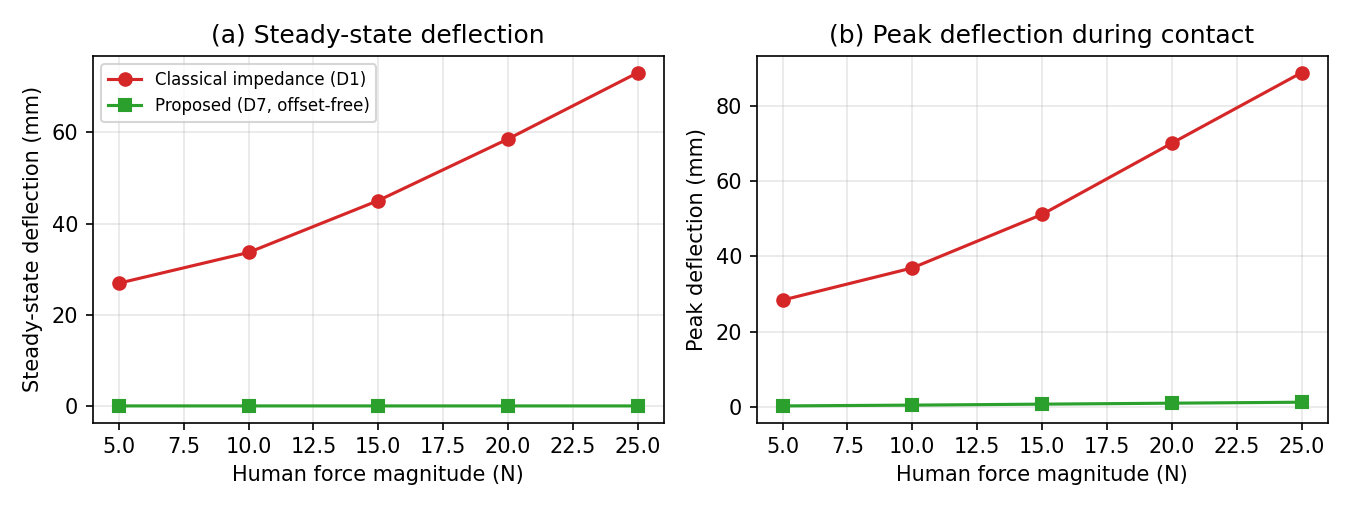
\includegraphics[width=\columnwidth]{figures/force_sweep.png}
\caption{Human-force magnitude sweep: steady-state (a) and peak (b) tip
deflection versus a sustained push, for classical impedance (D1, red)
and the proposed offset-free controller (D7, green). The proposed
steady-state deflection is invariant to force magnitude (0.021\,mm),
while classical impedance grows linearly.}
\label{fig:fsweep}
\end{figure}

% ----------------------------------------------------------
\section{Correction-Authority Robustness (Impedance-Backbone Ablation)}\label{sec:backbone}

Every controller in the main paper places the entire task-space
correction inside one box-constrained decision variable, $\Fmpc$: if it
is driven toward zero --- a tight $F_\text{max}$ bound, or a horizon step
whose predicted torque is unrealizable --- the commanded torque degrades
to the feedforward term $\tau_\text{ff}$ alone, i.e.\ zero corrective
stiffness. We evaluate an architectural ablation, \textbf{C8}, that
decouples baseline corrective stiffness from the optimizer: a fixed,
positively damped impedance law
\begin{equation*}
F_\text{bb}=K_\text{bb}e+D_\text{bb}\dot e,\qquad K_\text{bb}=300\text{ N/m},
\end{equation*}
is commanded on every MPC update independent of the QP output
($D_\text{bb}=2\zeta_\text{bb}\sqrt{K_\text{bb}}$, a nominal
unit-effective-mass tuning --- $\Laminv$ is generally anisotropic, so
this is not exact modal-critical damping), and the QP shapes only a
bounded additional correction $\Fmpc$ ($\|\Fmpc\|_\infty\le F_\text{max}$)
predicted through the backbone dynamics linearized at the current
configuration, $A_\text{cl}=A_d+B_d(\rho_k)G_\text{bb}$. If the QP's
output is driven to exactly zero for any reason, the commanded controller
retains this non-zero corrective stiffness instead of reverting to bare
feedforward. This is QP-independence, not actuator-limit independence:
the \textbf{total commanded torque is
$\tau=\tau_\text{base}+J_v^\top(F_\text{bb}+\Fmpc)$} --- $F_\text{bb}$ is
not optional and must be included in any torque-feasibility check ---
and C8 additionally applies the main paper's eq.~(9b) row at
\emph{every} horizon step rather than only the first, frozen at the
current configuration:
\begin{align*}
-\tau_\text{max}&\le\tau_\text{base}(0)+J_v^\top(q_0)
\bigl(F_\text{bb}+\Fmpck{i}\bigr)\\
&\le\tau_\text{max},\qquad i=0,\ldots,N-1,
\end{align*}
the frozen-Jacobian horizon-wide extension of (9b) --- not implied by
(9b)/(9c) alone, and specific to C8, not part of the default (C1--C7)
formulation. Freezing $J_v(q_0)$, $\tau_\text{base}(0)$ across the
horizon is a local approximation, not an exact prediction of future
torque feasibility. With this in place, the evidence below supports
robustness to loss of \textbf{additive QP correction authority}
specifically, not a blanket guarantee under arbitrary actuator saturation
or solver failure.

\textbf{Scenario and protocol.} Identical to Benchmark~I: 12\,cm
circular reference, 15\,N step push, 3 cycles / 24\,s, contact-window
metrics averaged over all three push events. We sweep the
corrective-force bound $F_\text{max}\in\{150,20,5,1,0\}$\,N, holding
every other parameter fixed, emulating progressively severe loss of
additive correction authority; $F_\text{max}=0$\,N is the limiting case
in which the QP contributes nothing.

\textbf{Results.} Under the normal protocol ($F_\text{max}=150$\,N), C8
matches C7 to measurement precision --- RMS/contact/peak/SS of
12.66/0.15/0.76/0.022\,mm vs.\ C7's 12.61/0.15/0.77/0.022\,mm (both
reproduced under the present codebase for a self-consistent comparison;
both agree with the main paper's Table~I C7 row to within a small
residual difference from an exact zero-order-hold correction applied
after that table was generated). The stress sweep is the key comparison:

\begin{table}[!t]
\caption{Correction-Authority Ablation: $F_\text{max}$ Sweep, RMS /
Peak (mm)}
\label{tab:backbone}
\renewcommand{\arraystretch}{1.0}
\footnotesize
\setlength{\tabcolsep}{3pt}
\begin{tabular}{lccccc}
\toprule
$F_\text{max}$ [N] & 150 & 20 & 5 & 1 & 0\\
\midrule
C7 -- RMS cont. & 0.15 & 0.15 & 317.6 & 414.0 & 424.4\\
C7 -- peak      & 0.77 & 0.76 & 412.3 & 552.5 & 560.8\\
\textbf{C8 -- RMS cont.} & \textbf{0.15} & \textbf{0.15} & \textbf{22.5} & \textbf{37.7} & \textbf{41.3}\\
\textbf{C8 -- peak}      & \textbf{0.76} & \textbf{0.76} & \textbf{29.8} & \textbf{47.9} & \textbf{51.6}\\
\bottomrule
\end{tabular}
\end{table}

\textbf{Analysis.} At $F_\text{max}\ge20$\,N there is enough headroom
that both controllers are unaffected and C8 costs nothing relative to
C7 --- the backbone's restoring term is exactly what the unconstrained
QP would already have produced. Below that, C7's contact-window RMS
jumps by roughly three orders of magnitude (0.15 $\to$ 424\,mm) the
moment the corrective force can no longer supply the needed authority:
with $\Fmpc$ forced toward zero, the commanded torque approaches bare
feedforward against the sustained push. \textbf{C8 degrades gracefully
instead}, settling at 22--41\,mm even in the $F_\text{max}=0$ limit ---
a 10--14$\times$ smaller error than C7 across the curtailed range, and
bounded rather than diverging. The impedance-equivalence and offset-free
statements of Theorems~1--2 of the main paper are proved for the standard
(non-backbone) realization; C8's additive term retains the same
offset-free mechanism (the $-\dhat$ centering trick is applied to
$\Fmpc$, not the backbone), but a formal re-derivation of the theorems
for the backbone-augmented closed loop is left to future work. This is
an architectural finding about how to \emph{deploy} the predictive
layer safely, complementary to and compatible with the energy-tank
layer of the main paper's Section~IV-C (which governs coupled-system
stability rather than QP-authority loss); it is reported here as a
self-contained ablation rather than folded into the main paper's
central narrative. Reproduced by
\texttt{stable\_backbone\_comparison.py --n-cycles 3}.

\begin{figure}[t]
\centering
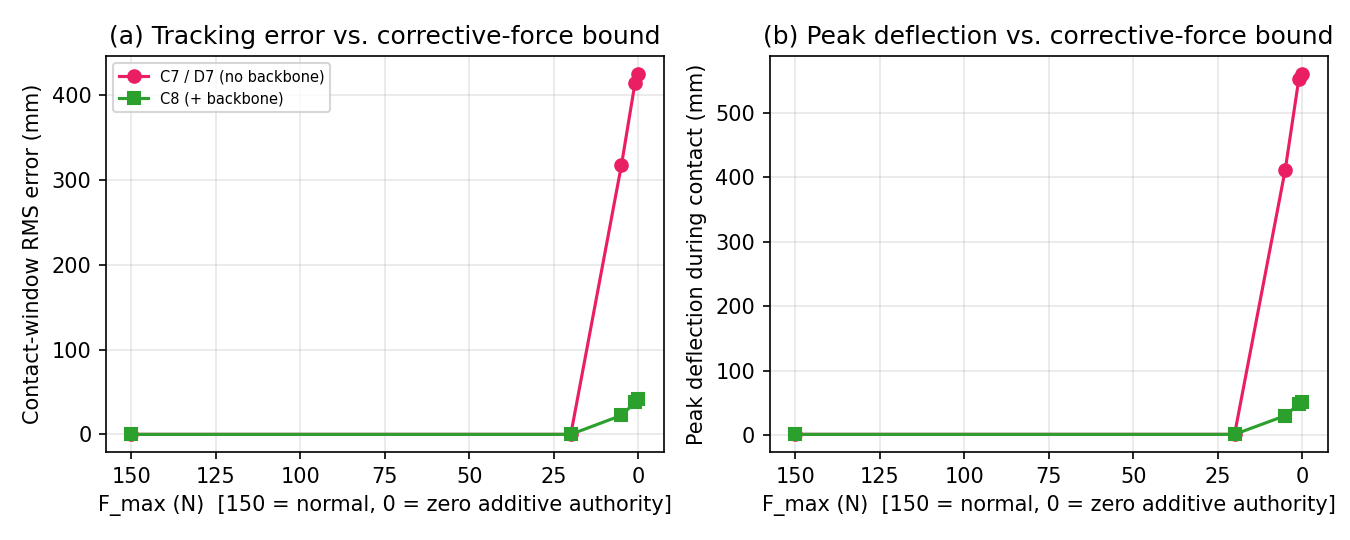
\includegraphics[width=\columnwidth]{figures/stable_backbone_comparison.png}
\caption{Correction-authority robustness ablation: contact-window RMS (a)
and peak deflection (b) versus the QP's corrective-force bound
$F_\text{max}$, for the proposed controller with (C8, green) and
without (C7, red) the impedance backbone. C8 degrades gracefully as
$F_\text{max}\to0$ while C7 collapses toward bare feedforward.}
\label{fig:backbone}
\end{figure}

\end{document}
